\documentclass[LSE,toc]{lsstdoc}

%% Journal abbreviations

\title[LSST Science Platform]{LSST Science Platform Vision Document}

\author{
M.~Juri\'c,
D.~Ciardi,
and
G.P.~Dubois-Felsmann
}

\setDocRef{LSE-319}
\date{2017-09-11}
\setDocUpstreamLocation{\url{https://github.com/lsst-dmsst/LSE-319}}

\setDocAbstract{%
This document defines and describes the ``LSST Science Platform'', a set of integrated web applications and services deployed at the LSST Data Access Centers (DACs) through which the scientific community will access, visualize, subset and perform next-to-the-data analysis of the data collected by the Large Synoptic Survey Telescope (LSST).
\\

These services can be broken down to three different aspects: a web \textbf{Portal}, designed to provide essential data access and visualization services through a simple-to-use website, a \textbf{JupyterLab} environment, that will provide a Jupyter Notebook-like interface enabling next-to-the-data analysis, and an extensive set of \textbf{Web APIs} that the users will be able to use to remotely examine the LSST data set using tools they're already familiar with.
\\

This document lays out the high-level vision for the aforementioned aspects and some associated backend services. It is intentionally brief, and meant to generally guide the flow-down of requirements and development product specifications, prioritization, and plans for the Agile development of the relevant elements of the DM system.

}

% Change history defined here. Will be inserted into
% correct place with \maketitle
% OLDEST FIRST: VERSION, DATE, DESCRIPTION, OWNER NAME
\setDocChangeRecord{%
\addtohist{}{2017-05-22}{Initial version}{Mario Juric}
\addtohist{1.0}{2017-09-11}{Approved in \href{https://project.lsst.org/groups/ccb/node/1762}{LCR-1013}}{Tim~Jenness}
%\addtohist{2}{yyyy-mm-dd}{Future changes}{Future person}
}

\begin{document}

% Create the title page
% Table of contents will be added automatically if "toc" class option
% is used.
\maketitle

\section{Preface}

The purpose of this document is to lay out the high-level vision for the \textbf{LSST Science Platform (LSP)}, a set of web applications and services through which the the scientific community will to access, visualize, interact with, and analyze LSST data holdings. With its companion document -- the Data Products Definition Document (\DPDD) -- it defines the high-level vision for LSST's end-user deliverables.
\\

To a future LSST user, this document should illustrate what will be made available to the science community through the LSST Data Access Centers. To LSST builders, it provides direction on how to flow down the LSST System Requirements Document (\LSR) to Data Management requirements (\DMSR) as they pertain to the end-user services provided at the LSST Data Access Centers.
\\

Though under strict change control, this is a \textbf\emph{living document}. LSST will undergo a period of construction  and commissioning lasting no less than seven years, followed by a decade of survey operations. To ensure their continued scientific adequacy, the high-level vision for LSST Science Platform will be periodically reviewed and updated.

\clearpage

\include{Introduction}
\section{User-facing Services}

\subsection{Portal Aspect\label{sec:portal}}

\begin{figure}
	\centering
	\scalebox{0.4}{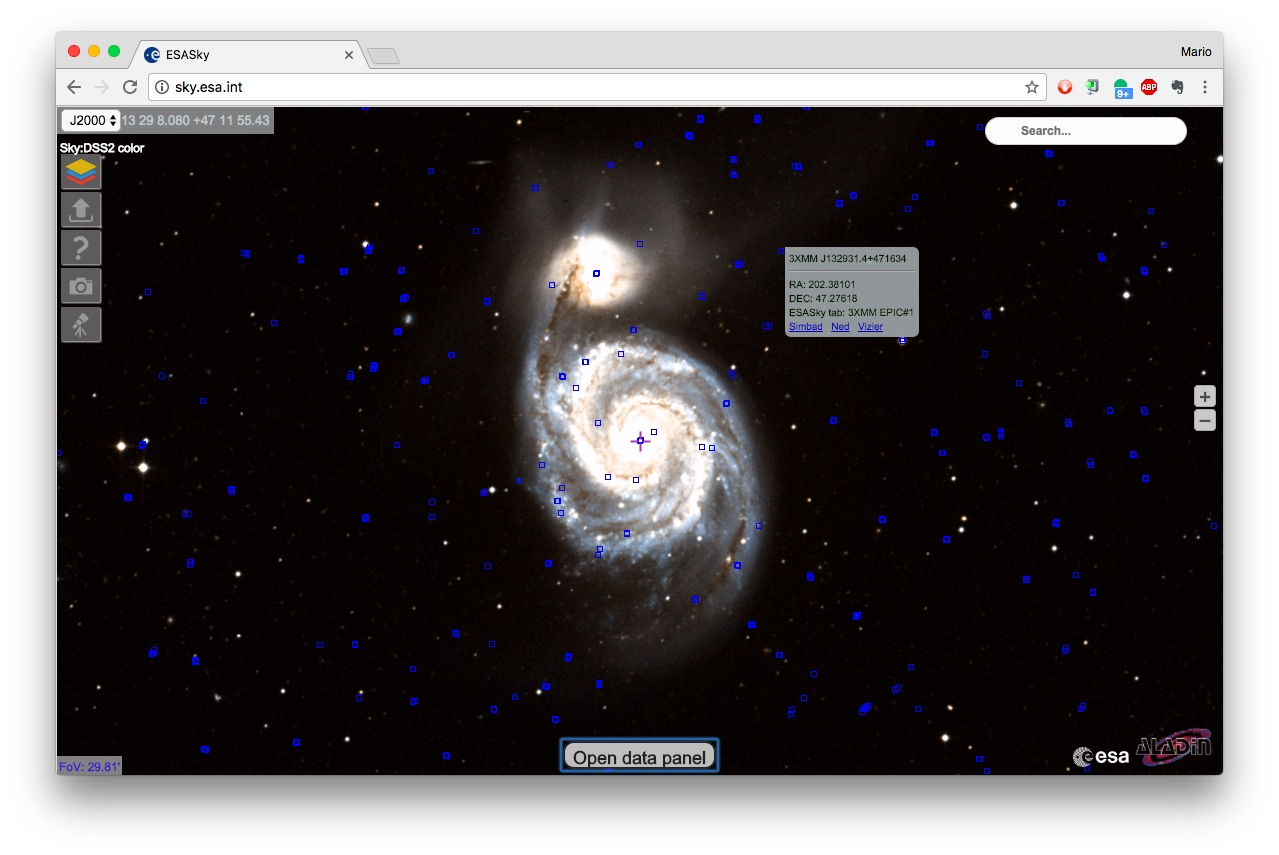
\includegraphics{images/fig-portal-esasky}}
	\caption{The "ESA Sky" web portal interface to ESA Archive holdings. The LSST portal user
		experience will support similar modern pan/zoom/select metaphor for exploration and visualization of the LSST data set.
		\label{fig:portalESA}}
\end{figure}

\begin{figure}
	\centering
	\scalebox{0.4}{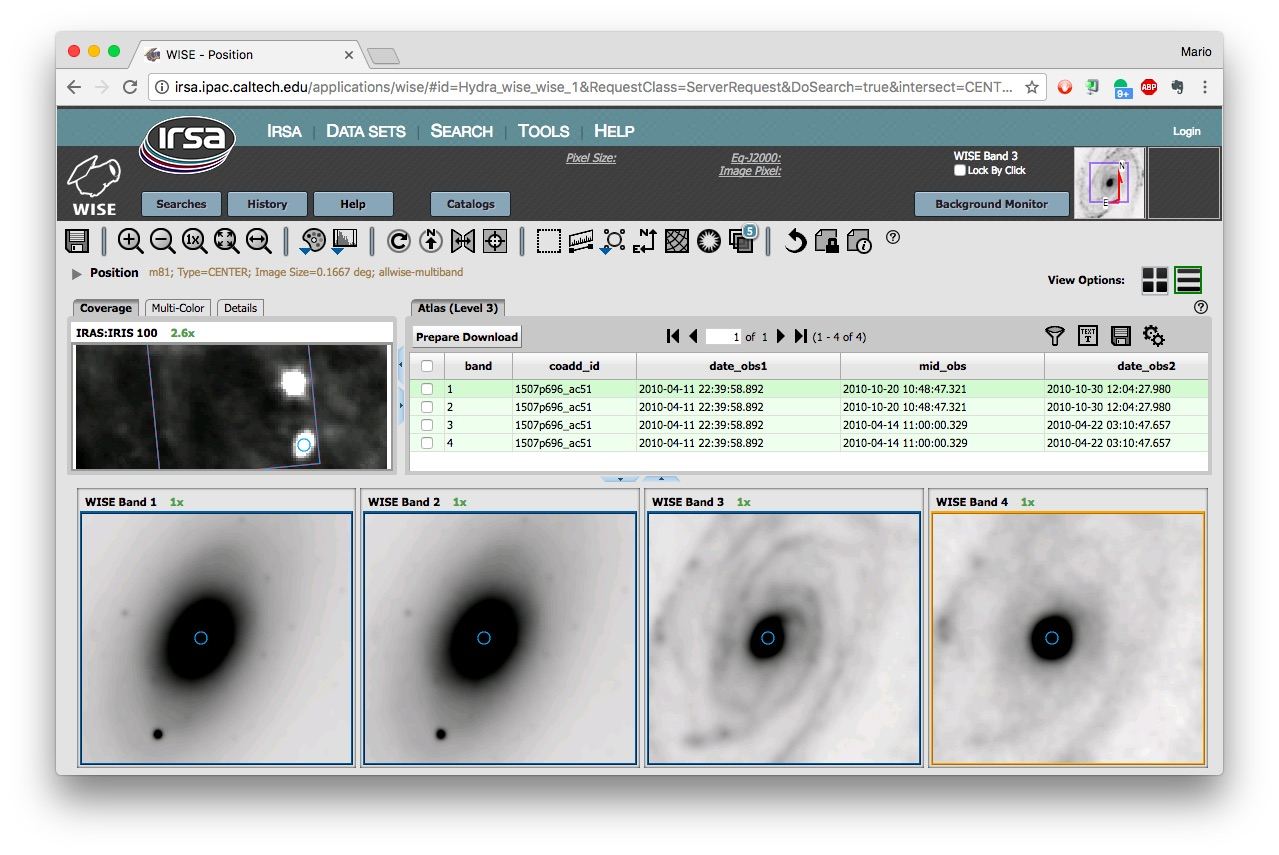
\includegraphics{images/fig-portal-irsa}}
	\caption{The web portal interface to the WISE data set at the Infra-Red Science Archive at IPAC. The LSST portal is being built by extending the Firefly toolkit that powers the IRSA/WISE archive.
		\label{fig:portalIRSA}}
\end{figure}

The \textbf{Portal Aspect} is a web portal designed to provide the essential data
access and visualization services through a simple-to-use website.  It is to
enable browsing and visualization of the available datasets in ways the
users are accustomed to at archives such as IRSA, MAST, or the SDSS archive.
To those we will add an enhanced level of interactivity in line with expectations for
then-contemporary archive portals (similar to that found today in ESASky and
the DECaLS Viewer). Examples of the types of user experiences to be offered
through the LSST portal are shown in Figures~\ref{fig:portalESA}~and~\ref{fig:portalIRSA}.

Through the Portal, the users will be
able to view the LSST images, request subsets of data (via simple forms or
ADQL queries), store the results of such queries to their personal
workspaces, as well as download them. The Portal will also make it possible to
construct commonly requested plots, and generally explore the
LSST dataset in a way that allows the users to identify and access (subsets of)
data required by their science case.

Virtually all LSST users will use the Portal as their first point of entry to
access and explore the LSST data set. When developing the Portal,
we will therefore \textbf{emphasize the user experience and exploratory
capabilities}, over analysis features. The latter are expected to be more
directly satisfied by the Notebook Aspect.

\subsection{Notebook (JupyterLab) Aspect\label{sec:jupyter}}

\begin{figure}
	\centering
	\scalebox{0.6}{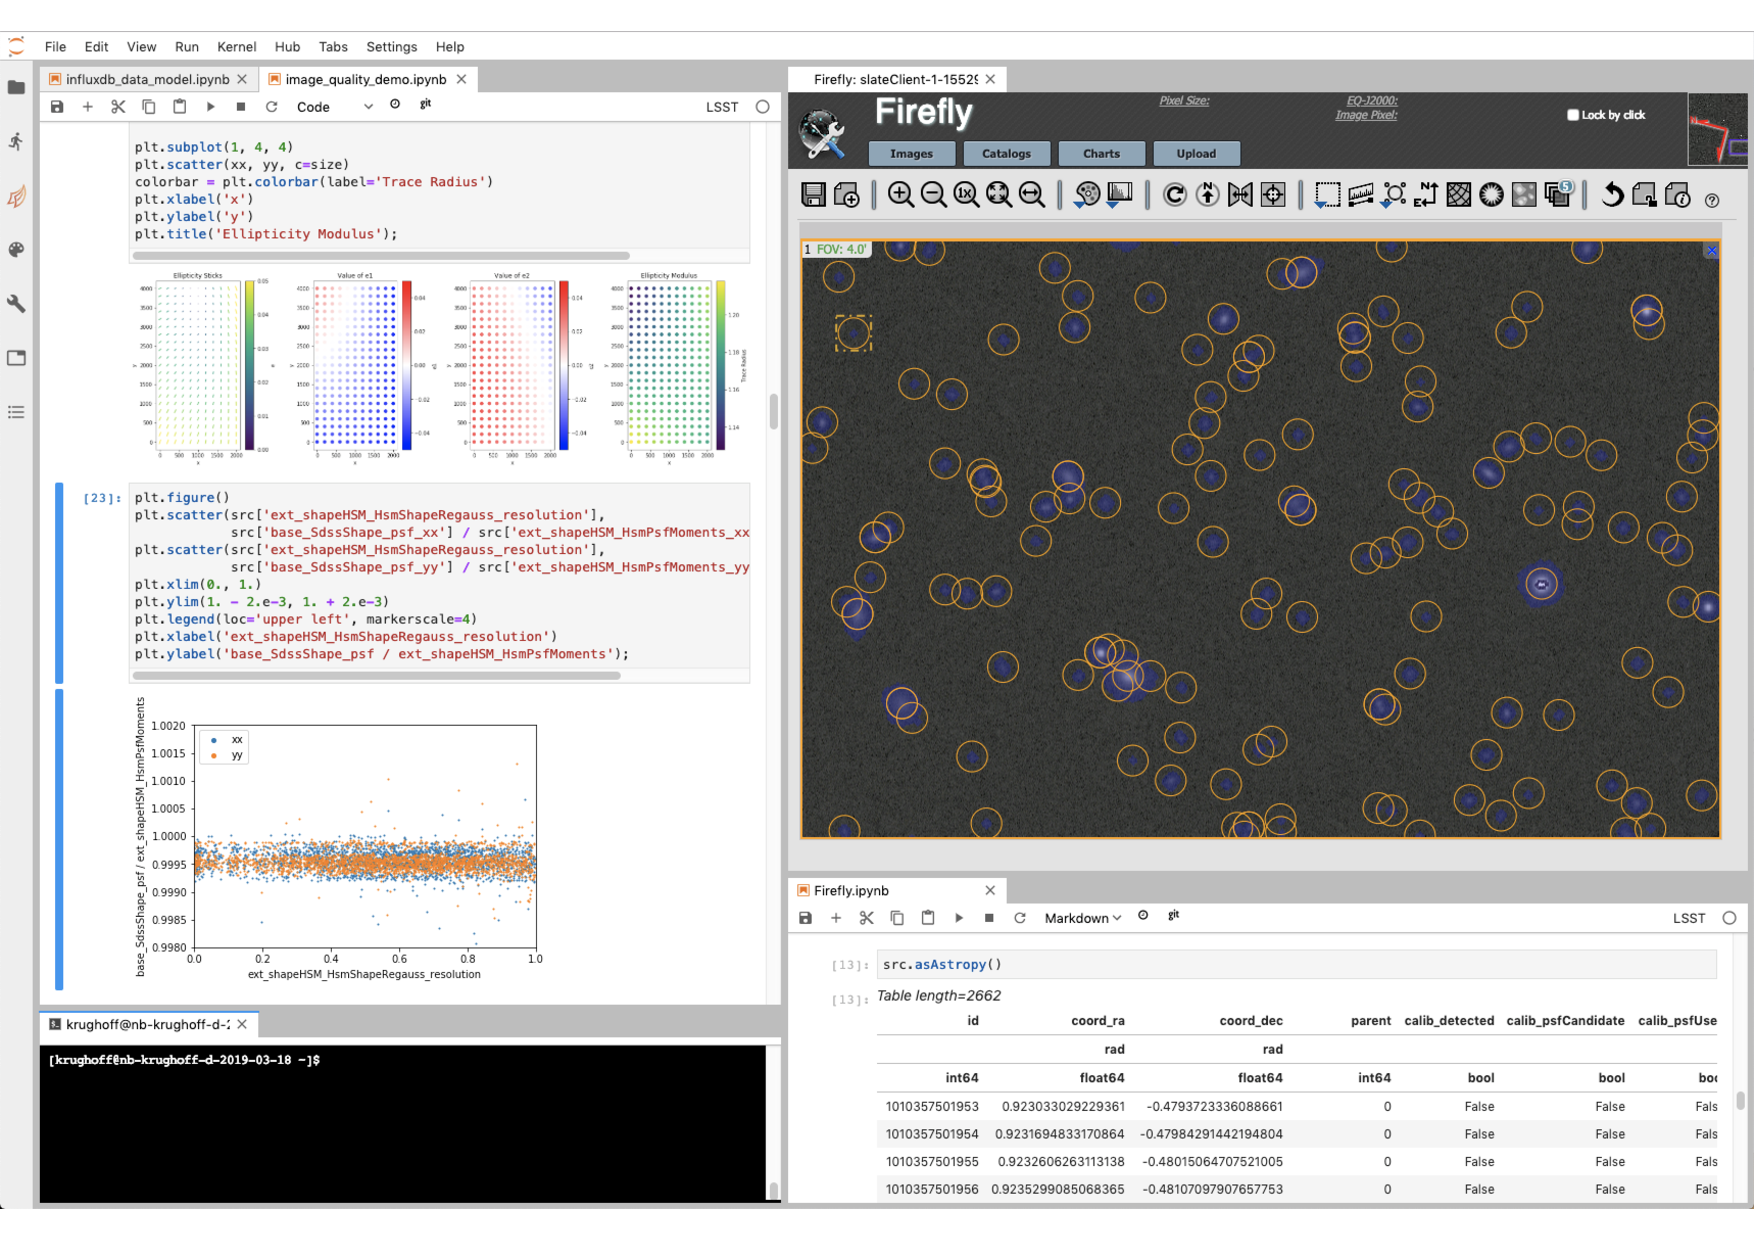
\includegraphics[scale=0.9]{images/fig-notebook-imagequality}}
	\caption{A screen capture of the Notebook interface running LSST image processing code within a notebook. \label{fig:JupyterLab}}
\end{figure}

The \textbf{Notebook Aspect}
%, based on the Jupyter family of technologies (such as JupyterHub and JupyterLab), 
will be provided to allow for more sophisticated data selection, analysis, and creation of added value \textit{User Generated} data products. 
A screen capture of a mature prototype of the Notebook Aspect is shown in Figure~\ref{fig:JupyterLab}.

The Notebook Aspect user experience will be nearly identical to working with
Jupyter notebooks locally, except that computation and analysis will occur
at resources provided at the LSST Data Access Center.
This is an
implementation of the ``bringing analysis to the data'' paradigm: rather
than imposing the burden of downloading, storing, and processing (large)
subsets of LSST data at their home institutions, we will enable our users to
bring their codes to and perform their analysis at the LSST DAC.  We expect
this will reduce the barrier to entry and shorten the path to science for
the LSST science community.

We will provide JupyterLab instances to LSST users in an environment carrying a
library of preinstalled commonly used and useful software tools:
Astropy, the LSST science pipelines, Anaconda Scientific Python Distribution, the PyViz visualization toolkit, and others. 
The users will be able to upload and install their own tools as well.
Non-trivial shared computing cluster resources will be accessible through this environment as well, enabling the generation of \textit{User Generated} data products.

% Add something about writing glue code to make it easy to submit jobs, and how Notebooks will be the primary user interface to the backend batch system...

The Notebook Aspect of the science platform will play a key role in commissioning,
quality assessment, and science validation of the as-built system.
It will be the primary
method of performing interactive analysis of acquired data (e.g., adjusting and executing
prepared notebooks driving commissioning tasks), as well as commanding
the batch resources to execute larger processing tasks.
Due to this, we expect the
Notebook Aspect to reach maturity earlier than the others, and certainly in time for
commissioning.

% Data sets acquired during commissioning, as well as precursor and simulated data sets processed for quality assessment and science validation while construction is ongoing, will appear in the commissioning workspace, ready for operator analysis using tools and

\subsection{Web API Aspect\label{sec:apis}}

\begin{figure}
	\centering
	\scalebox{0.4}{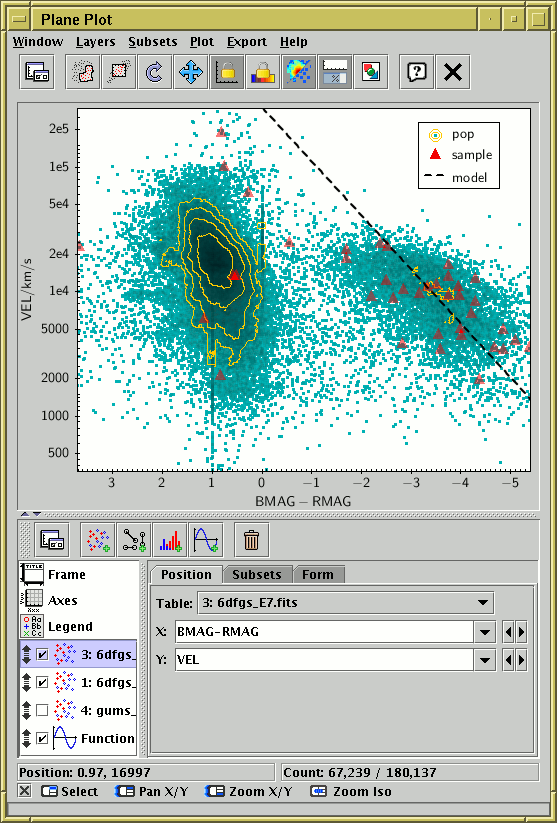
\includegraphics[scale=0.7]{images/topcat-StackPlotWindow}}
	\caption{A screen capture of Tool for OPerations on Catalogues And Tables (TOPCAT), that is capable of remotely accessing catalogs using VO protocols. Tools such as these will be able to directly access the data sets served by the LSST DACs (figure credit: Mark Taylor, \url{http://www.star.bris.ac.uk/~mbt/topcat/sun253/sun253.html}).
		\label{fig:toolsTOPCAT}}
\end{figure}

Backend Platform services -- such as access to
databases, images, and other files -- will be exposed to the public Internet through
machine-accessible web APIs.
These will serve the data using community-accepted
formats and protocols, making it easy to remotely access the LSST data and DAC	
services.
Furthermore, to ensure maximal exposure of the DAC services through the Web APIs,
the other two Aspects of the Platform --- Portal and Notebook --- will
internally access the LSST datasets using the same Web APIs to the greatest extent possible.

Exposing the LSST data through Virtual Observatory interfaces plays a particularly important role.
This will allow the discoverability of LSST data products from within the Virtual Observatory,
and federation of the LSST data set to other archives.
It will also enable the use of widely utilized tools such as TOPCAT or DS9 by the end-users,
further lowering the barrier to access to LSST data, and shortening the path to science.
It will also allow these tools to be used in commissioning,
easing the way for scientists new to the LSST environment to access the data and make meaningful
contributions to this time-compressed activity.

LSST will follow a ``VO-first'' strategy, using IVOA-standard interfaces wherever practical,
though we may also provide some services using custom protocols in areas where relevant standards have not yet been developed.
LSST will actively participate in the IVOA community, and will propose evolutions of standards when we find problems and where we feel that our custom work could be of broader benefit to the community.
We will also use our engagement with the IVOA to ensure that we are following mainstream interpretations of the standards and to maintain contact with the authors of client software such as TOPCAT.

Additional details on the standards to be supported are provided below.

\subsection{Integrated environment}

All the Aspects of the LSST Science Platform are intended to be \textit{well integrated}, enabling a seamless workflow so the users will be able to move back and forth between them as needs dictate.
The aim is to enable a user to find or create data in one Platform Aspect, and view or analyze that data in another.

As an example of how these connections can aid a user in exploring the LSST data, data queries will be shareable across the Portal, Notebook, and Web API Aspects.
This will allow a user to build a query using the Portal's TAP query UI component, view the (possibly preliminary) results by browsing them in place in the Portal, and then access the final results from a JupyterLab notebook or a remotely connected client (e.g., TOPCAT) for further analysis.
The reverse flow will also be enabled; a user can code and submit a complex SQL query in the Notebook, and then browse and visualize the results in the Portal.

By making the environments integrated, we allow for a shallower learning curve and a gradual transition to more complex environments at the point they are needed.
For example, a user may begin interacting with the LSST dataset using the Portal Aspect but may ultimately reach the limitations of the selection and analysis tools it provides.
The integrated nature of the platform will allow such a user to switch to the Notebook Aspect, and continue working on the data analysis started in the Portal.
There, they will be able to import the analysis artifacts (e.g., catalog subsets) as standard Python objects (e.g., as astropy.table).

\subsection{Next to Data Processing\label{sec:n2d}}
Many LSST science cases will require analysis of the full LSST Object and/or Source tables; subsetting and downloading reduced catalogs will not suffice for science that requires, for example, fitting and computing features of light curves for large numbers of Objects, creating maps of stellar density, or training machine learning models.
The LSST Object table alone will be $\approx$~50TB for Data Release 1 and $\approx$~300TB for Data Release 11 at the close of the 10-year survey.
The LSST Science Platform will enable user-driven large-scale search and analysis capabilities of the LSST data by providing a \textit{Next-to-Data} processing environment, allowing users to bring their analysis to the data.
This environment will be supported by backend services, as described in \ref{sec:backend}

\subsection{Supporting Collaborative Work\label{sec:collab}}

The LSST Science Platform will provide support for collaborative work at two levels:
\begin{itemize}
	\item \textbf{Shared workspaces}: Creation and sharing of data sets --- catalogs, images, queries, and other data products --- within either pre-defined or dynamically-created groups (e.g., a research group at a university, or a large science collaboration).
Such groups would have access to a shared virtual ``workspace'' within the LSST DAC.
This workspace will include shared files, shared catalogs (stored in user databases) as well as computing cycles allocated to the group as a whole.
This shared workspace will be equally ``visible'' from all three Aspects of the platform --- e.g., uploads to the workspace will be possible either through a form in the Portal, POSIX-style file access from JupyterLab, or using an external file transfer client via WebDAV or VOSpace.

	\item \textbf{Shared editing}: Although we have no formal requirement to provide shared editing capabilities, we envisage supporting ``Google Docs''-like collaborative editing, visualization, and data analysis capabilities, via the integration of 3rd-party tools, \emph{if and when these technologies become available in upstream products}.
	% At present, collaborative editing is on the development roadmap for Jupyter Notebooks, and will be included into our Notebook Aspect as it reaches production quality.
\end{itemize}

The levels of support for collaboration described above are responsive to the large majority of user needs identified by end-user focus groups in R\&D. At the same time, they minimize the technical risks by leveraging widely used and well understood technologies (SDSS-like MyDB user databases, backend authentication \& authorization mechanisms, VO protocols, Jupyter).

\section{Backend Services\label{sec:backend}}

The user-facing aspects of the LSST Science Platform will be built on top of a number of backend services that can roughly be divided into three categories: \textbf{database services}, \textbf{file services}, and \textbf{batch computing} services (bottom row of Figure~\ref{fig:layeredLSP}). The details of these services are described in the Data Management Design Document (\citeds{LDM-148}) and other associated documents; here, we only provide the high-level guidance as to the capabilities which these services will need to expose to the user (through the three aspects).

\subsection{Database Services}

Key LSST catalogs, both for \textit{Prompt} and \textit{Data Release} data products, will be stored in relational databases and made available for querying by users using the Structured Query Language (SQL) as well as Astronomical Data Query Language (ADQL). These products, and expectations surrounding their schemas, are further described in the \DPDD.

Besides serving the LSST catalogs, LSST databases will also provide a per-user database space allocation. Within this allocation, end-users (including groups) will be able to store selected or transformed subsets of the LSST dataset, or upload related datasets for joining to the LSST dataset. The size of this allocation is determined by the \SRD requirement to provide 10\% of total LSST computing and storage resources to LSST users.

\subsection{File Services}

LSST Science Platform will also provide a per-user file space allocation. End-users (including groups) may use this allocation to upload code, store selected or transformed subsets of the LSST dataset (e.g., images), and in general keep files needed to support their data analysis work. Note that some of this space may be provided in form of an object store, rather than a file system with POSIX-like semantics.

The size of this allocation is determined by the \SRD requirement to provide 10\% of total LSST computing and storage resources to LSST users.

\subsection{Batch Computing Services}

Analysis performed through the Portal, JupyterLab, and Web API will be served by a shared computing cluster. This cluster will be managed by a workload management system that ensures resources are allocated to individual users or groups based on pre-determined operational policies. The size of the batch computing resource is determined by the \SRD requirement to provide 10\% of total LSST computing and storage resources to LSST users.

The users will be able to launch jobs on the batch computing cluster primarily utilizing the APIs exposed through the JupyterLab and Web API aspects of the LSST Science Platform. Some functionality exposed through the Portal may potentially utilize the batch computing cluster as well.

%\subsection{Overall User Experience}
%
%At start of operations,
%this computing cluster will number 2,400 cores (approximately 18 TFLOPs),
%with 4 PB of file and 3 PB of database storage (numbers for the U.S.  DAC).
%These will be shared by all users, the number of whom we’re estimating in
%the low thousands.
%
%Not all users will be accessing the computing cluster concurrently; though
%difficult to predict with accuracy because of a lack of direct comparables,
%an estimate on order of a ~100 concurrent users is likely reasonable.  This
%would translate to typical allocations of ~20 cores per user, sufficient to
%enable preliminary end-user science analyses (working on catalogs, smaller
%number of images) and creation of some added-value (User Generated) data products.
%A good analogy is one of being given a server with a few TB of disk, few TB
%of database storage, that is co-located next to the LSST data, and with a
%chance to use tens to hundreds of cores for analysis (depending on system
%load).
%
%Note that for larger endeavors (e.g., pixel-level reprocessing of the entire LSST
%dataset), the users will be steered towards resources beyond the LSST DACs
%(e.g., national supercomputing centers, university computing centers, or the
%public cloud).
%
%\subsection{Integrated aspect: the User Workspace}
\section{Development Methodology and Prioritization Guidance\label{sec:methdology}}

\subsection{Iterative Development Leveraging Existing Technologies }

The services constructed for the LSST Science Platform will be developed following the iterative Agile methodology. While most of LSST software development follows this approach, adopting it is especially advantageous for user-facing services. There, iterative development and nearly continuous stakeholder feedback can provide guidance as to the details of features to be implemented, the continued validity of the approach taken, and the expected focus of intermediate milestones.

The development of the Portal, JupyterLab, as well as Web API aspects will start from significant existing code bases and prior art. This is a deliberate approach designed to minimize technological risk and leverage end-user familiarity with these interfaces. The latter also reduces the barrier to user adoption of the products eventually delivered for LSST.

The \textbf{Portal} is based on existing, production quality, archive portal interface developed at IRSA/IPAC -- the \emph{Firefly} toolkit. The primary challenge is integrating the existing Firefly code, and updating the user experience to conform to anticipated user expectations (e.g., supporting all-sky maps and pan/zoom/click-type exploration). Consistent with the general philosophy, DM should look at achieving the necessary upgrades by re-using existing well-known libraries and tools (e.g. Aladin Lite).

The \textbf{JupyterLab} environment will be based on the open-source JupyterLab product delivered and maintained by the Jupyter team. The development of the JupyterLab aspect of the LSST Science Platform will focus on deployment and integration with the LSST-specific backend services and other aspects of the platform, rather than developing new or radically different features within the JupyterLab product.

Finally, the \textbf{Web API} aspect is envisioned as implementing existing, widely-adopted, community protocols (e.g. such as those from Virtual Observatory suite of protocols and standards). Similarly to other aspects, it will benefit from leveraging existing codes and libraries wherever appropriate.

\subsection{Prioritization Guidance}

Here we give some overall feature prioritization guidance, to enable the construction of initial (mostly functional) requirements and intermediate development milestones.

Portal aspect:
\begin{enumerate}
	\item Deployment of the initial Firefly back-end within the (prototype) LSST Data Access Center at NCSA.
	\item Integration of the initial Firefly front- and back-ends with LSST Science Platform backend services. For example, this includes the authentication and authorization mechanisms, relational databases, file stores, etc.
	\item User experience improvements, such as addition of all-sky maps with pan/zoom/select navigation metaphors, modernization of the look-and-feel, streamlining of the UI and deprecation of rarely used widgets. \textbf{Once this level of functionality is met (at scale), the Portal aspect will have achieved the minimum level of viability for deployment to operations}.
	\item Improved user workflow integration with other aspects of the LSST Science Platform. For example, it should be possible to begin data exploration in the Portal (e.g., by interactively selecting data sets) and seamlessly transfer the sub-selected catalogs and images to the JupyterLab environment for further, more complex, analysis using provided Python libraries.
	\item Addition of new widgets and abilities to the Portal, that address most requested and broadly useful end-user needs.
	\item Widget-level integration with JupyterLab.
\end{enumerate}

JupyterLab aspect:
\begin{enumerate}
	\item Deployment of the initial JupyterLab product within the (prototype) LSST Data Access Center at NCSA.
	\item Integration of the JupyterLab product with LSP backend services, most notably authentication and authorization, user management, databases, and file stores. \textbf{Once this level of functionality is met (at scale), the JupyterLab aspect will have achieved the minimum level of viability for deployment to commissioning and operations}.
	\item Development of libraries and utilities to ease the submission of user-written code from Jupyter notebooks to the batch compute system.
	\item Creation and curation of a library of 3rd party code that will be made available to LSP end-users.
\end{enumerate}

Web APIs:
\begin{enumerate}
	\item Development and deployment of initial data access APIs needed to satisfy the back-end needs of the Portal and JupyterLab aspects. These may not yet "speak" the final, standards-compliant, protocols.
	\item Integration of the Web API aspect with LSP backend services, most notably authentication and authorization, user management, databases, and file stores.
	\item Deployment of critical protocols (including SCS, TAP, SIA, SODA, VOEvent streaming support, and VO Registry support) at commonly-encountered levels of standards compliance (eg., the most commonly used ADQL features). \textbf{Once this level of functionality is met (at scale), the Web API aspect will have achieved the minimum level of viability for deployment to operations}
	\item Deployment of standards-compliant protocols throughout the Web API aspect, and integration with all other elements of the Platform.
\end{enumerate}

It is assumed that the development of backend services will be driven by the needs of the front-end aspects.
\section{Design for Evolution\label{sec:evolution}}

This document captures DM's response to our best estimate of what the expectations of LSST users are likely to be, starting with LSST Commissioning and through the first few years of LSST Operations.

Through a decade of operations, it is likely that both the user expectations will change, as well as the technologies available to respond to them.
For example, the emergence of Jupyter as the dominant mode of remote data analysis in the astronomical community has caused the present vision and design of the LSST Science Platform to be markedly different than the original conceptual design of the Science User Interface and Tools (LDM-131).
There is no reason to believe that similar shifts will not happen in Operations as well.

The LSST will therefore proactively design the LSST Science Platform services with such an evolution in mind, to a degree permitted by the available budget and schedule constraints.
An example of such \textbf\emph{design for evolution} is the concept of loosely coupled aspects itself (the Portal, Notebook, and Web APIs), that all expose different views of the same underlying data model and workspace.
Design principles like these will allow for additions of new LSST Science Platform Aspects (e.g., a different Jupyter-like technology, should one emerge), replacements of Aspects (e.g., migrating to a different Portal technology), as well as retirement of Aspects that are not widely used.

\clearpage

\bibliography{lsst}

\end{document}
